\title{Simulation using Hamiltonian Monte Carlo}
\author{
        Ho Chung Leon  Law \\
            \and
        Nathan Cunningham\\
}
\date{\today}

\documentclass[11pt]{article}
\usepackage{amsmath}
\usepackage{algorithm}
\usepackage{algpseudocode}
\usepackage{graphicx}
\usepackage{hyperref}
\usepackage[a4paper,bindingoffset=0.2in,%
            left=1in,right=1in,top=1in,bottom=1in,%
            footskip=.25in]{geometry}
\begin{document}
\maketitle

\begin{abstract}
In this report we aim to examine the properties of Hamiltonian Monte Carlo, implement it in the R coding language, and compare its effectiveness to another method of monte carlo simulation. \ldots
\end{abstract}
\newpage
\section{Introduction}
Hamiltonian Monte Carlo (HMC) is a Markov Chain Monte Carlo (MCMC) method for simulating a random sample from a probability distribution which may not be feasible to simulate from directly. While the method was first proposed by Duane et al\cite{duane}, we focus primarily on the more statistically-orientated paper by Neal\cite{neal}.
\subsection{Aim}
Our aims in this report are to: Implement Hamiltonian Monte Carlo in the R coding language; examine the impact of the tuning parameters, $\epsilon$ and $L$, and methods of choosing these; compare Hamiltonian Monte Carlo to the Metropolis-Hastings (MH) algorithm.


\subsection{Motivation}
In cases of a multi-modal distribution many MCMC methods, including Metropolis-Hastings, can tend too much towards a local maximum and fail to explore the sample space. Hamiltonian Monte Carlo aims to get over this issue.
(comparison graphics of MH and HMC exploring sample space)

\section{Hamiltonian dynamics}
The Hamiltonian equations model the evolution of a particle in a frictionless system over time, $t$, given its momentum, $p$, and position, $q$. The Hamilton equation consists of the potential energy of the particle, $U(q)$, and the kinetic energy, $K(p)$, and in Hamiltonian Monte Carlo is usually written as
\begin{equation}
H(q,p) = U(q) + K(p)
\end{equation}
This system evolves according to the following differential equations:
\begin{equation}
\frac{dq_{i}}{dt} = \frac{\delta H}{\delta p_{i}}
\end{equation}
\begin{equation}
\frac{dp_{i}}{dt} = \frac{-\delta H}{\delta q_{i}}
\end{equation}



\subsection{Properties of Hamiltonian dynamics}

\paragraph{Reversibility}
\paragraph{Volume preservation}
\paragraph{Conservation of the Hamiltonian}
\paragraph{Symplecticness}
\subsection{The Leapfrog}
In order for the Hamiltonian dynamics to be programmed the time involved needs to be discretised. This can be done via Euler's equations (but some problems here) and is implemented using the leapfrog.
First advance the momentum by one half-step:
\begin{equation}
p_{i}(t+\epsilon/2) = p_{i}(t) - (\epsilon/2)\frac{\delta U}{\delta q_{i}}(q(t))
\end{equation}
then advance the position by a full-step using the updated momentum:
\begin{equation}
q_{i}(t+\epsilon) = q_{i}(t) - (\epsilon)\frac{p_{i}(t+\epsilon/2)}{m_{i}}
\end{equation}
And finally advance the momentum one half-step using the updated position:
\begin{equation}
p_{i}(t+\epsilon) = p_{i}(t+\epsilon/2) - (\epsilon/2)\frac{\delta U}{\delta q_{i}}(q(t+\epsilon))
\end{equation}
Iterate over this process $L$ times.

\section{Hamiltonian Monte Carlo}
In statistical mechanics the canonical distribution, given an energy function $E(x)$, can be expressed as
\begin{equation}
P(x) = \frac{1}{Z}exp(-E(x)/T)
\end{equation}
where $T$ is the temperature of the system (which we can assume as 1) and $Z$ is a normalising constant. Thus, we can convert our distribution $P(x)$ to a canonical distribution by setting the energy function, $E(x)$ to $-logP(x)-logZ$

Given that the Hamiltonian has been defined as $H(q,p) = U(q) + K(p)$ the joint density is given by
\begin{equation}
P(q,p) = \frac{1}{Z}exp(-H(q,p)/T)
\end{equation}
\begin{equation}
P(q,p) = \frac{1}{Z}exp(-U(q)/T)exp(-K(p)/T)
\end{equation}
Thus, p and q are independent and each have canonical distributions with energy functions $U(q)$ and $K(p)$. We set the variable $q$ to represent our variables of interest, and we introduce the variable $p$ to represent momentum to allow the Hamiltonian dynamics to operate. We can express the posterior distribution, $U(q)$, as a canonical distribution with a potential energy function defined as:
\begin{equation}
U(q) = -log[\pi(q)L(q|D)]
\end{equation}
For each iteration of the leapfrog we can intialise our momentum variable randomly from a distribution. Given that p and q are independent we can sample p from any distribution we like. Typically we choose p to have a zero-mean Gaussian distribution. Usually each of the $i$ components of p are assumed to be independent with variance $m_{i}$. Thus, the kinetic energy function producing this distribution is
\begin{equation}
K(p) = \sum_{i=1}^{d} \frac{p_{i}^{2}}{2m_{i}}
\end{equation}
Given the random initialisation of $p$ we then allow Hamiltonian dynamics to run for L steps to update $p$ and $q$ as appropriate. The new state is then accepted as the next state of the Markov chain with probability
\begin{equation}
min\{1,exp(-H(q^{*},p^{*})+H(q,p))\} = min\{1, exp(-U(q^{*}+U(q)-K(p^{*}+K(p))\}
\end{equation}
otherwise the next state is the same as the current state.

\begin{algorithm}
\caption{Hamiltonian Monte Carlo}\label{euclid}
\begin{algorithmic}[1] 
\State Select an initial $q$ 

\State $p\sim \mathcal{N}(0,\Sigma)$
\State Given $(q,p)$ Simulate Hamiltonian dynamics using the leapfrog for $L$ steps with $\epsilon$ to find $(q^{*},p^{*})$ 
\State Negate $p$ to ensure reversibility 
\State Accept $(q^{*}, p^{*})$ as the next step in the Markov chain with probability (M prob) 
\State Otherwise accept next step as $(p,q)$ 
\end{algorithmic}
\end{algorithm}

\subsection{Choice of $L$ and $\epsilon$}
The HMC method is sensitive to the user-tuned parameters $L$ and $\epsilon$. In particular, if L is too small, the algorithm devolves to random walk behaviour as the random samples highly correlated. Conversely, if L is too large it is computationally wasteful.
\section{Comparisons}
\subsection{Bivariate Gaussian simulation}
We first of all compared the effectiveness of the HMC method
\begin{figure}[H]
\center
  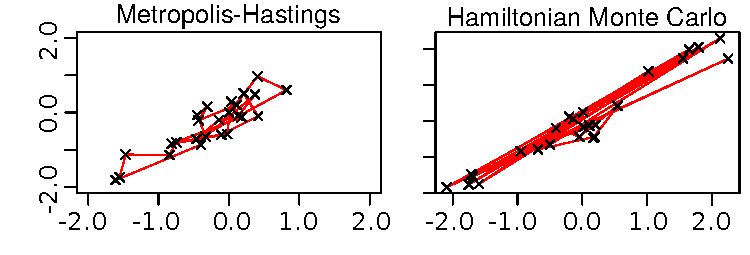
\includegraphics[width=5in]{images/MHvsHM_explore.pdf}
\caption{The trajectory of a bivariate Gaussian distribution simulated with zero-mean and marginal $\sigma$ of 1, and $\rho$ of 0.95.}
\end{figure}


\begin{figure}[H]
\center
  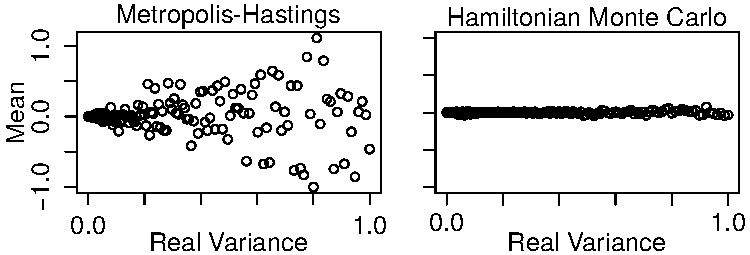
\includegraphics[width=5in]{images/MHvsHM_var.pdf}
  \caption{Mean}
\end{figure}
\subsection{High-dimensionality}
\begin{figure}[H]
\center
  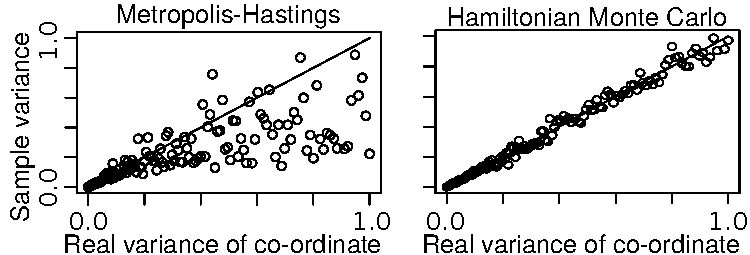
\includegraphics[width=5in]{images/MHvsHM_varcoord.pdf}
  \caption{A comparison of the real and observed variance of a highly-dimensional mutivariate Gaussian.}
\end{figure}
\subsection{Choices of $\epsilon$ and L}


\subsection{No U-turn sampler (NUTS)}
The No U-turn sampler\cite{NUTS} is an implementation of Hamiltonian Monte Carlo which aims to avoid the need for the user to manually specify $L$ and $\epsilon$
\cite{rstan}
\subsection{Normal mixture models}
We compared the performance of our model to that of the Metropolis-Hastings algorithm and the NUTS method, as implemented in RStan

\begin{thebibliography}{9}

\bibitem{neal}
  Neal R.M.,
  \emph{MCMC using Hamiltonian dynamics},
  Chapter 5 of the Handbook of Markov Chain Monte Carlo,
  2012.
  
\bibitem{duane}
  Duane,S., Kennedy,A.D., Pendleton,B.J., \& Roweth,D.,
  \emph{Hybrid Monte Carlo }
  Physics Letters B, 195(2) 216-222, 1987.

\bibitem{NUTS}
  Hoffman,M.D., Gelman,A.,
  arXiv:1111.4246v1.
  
\bibitem{rstan}
  RStan, \url{http://mc-stan.org/interfaces/rstan.html}

\end{thebibliography}
\end{document}
